\documentclass{article}
\usepackage[utf8]{inputenc} %кодировка
\usepackage[T2A]{fontenc}
\usepackage[english,russian]{babel} %русификатор 
\usepackage{mathtools} %библиотека матеши
\usepackage[left=1cm,right=1cm,top=2cm,bottom=2cm,bindingoffset=0cm]{geometry} %изменение отступов на листе
\usepackage{amsmath}
\usepackage{graphicx} %библиотека для графики и картинок
\graphicspath{}
\DeclareGraphicsExtensions{.pdf,.png,.jpg}
\usepackage{subcaption}
\usepackage{pgfplots}
\usepackage{array}
\usepackage{pgfplots}
\usepackage{multirow}
\usepackage{float}

\begin{document}
% НАЧАЛО ТИТУЛЬНОГО ЛИСТА
\begin{center}
    \Large
    Федеральное государственное автономное \\
    образовательное учреждение высшего образования \\ 
    «Научно-образовательная корпорация ИТМО»\\
    \vspace{0.5cm}
    \large
    Факультет программной инженерии и компьютерной техники \\
    Направление подготовки 09.03.04 Программная инженерия \\
    \vspace{1cm}
    \Large
    \textbf{Отчёт по лабораторной работе №5} \\
    По дисциплине «Математическая статистика» (четвёртый семестр)\\
    Оценивание параметров двумерной случайной величины\\
    \large
    \vspace{8cm}

    \begin{minipage}{.33\textwidth}
    \end{minipage}
    \hfill
    \begin{minipage}{.4\textwidth}
    
        \textbf{Студент}: \vspace{.1cm} \\
        \ Дениченко Александр\\
        \ Разинкин Александр\\
        \ Соколов Анатолий\\
        \textbf{Практик}:  \\
        \ Милованович Екатерина Воиславовна
    \end{minipage}
    \vfill
Санкт-Петербург\\ 2024 г.
\end{center}
\thispagestyle{empty}

% КОНЕЦ ТИТУЛЬНОГО ЛИСТА 
\newpage
\section*{Цель работы}
Цель работы состоит в построении оценок математических ожиданий и дисперсии случайных величин, входящих в систему, а также оценок корреляционного момента и коэффицента корреляции.
\section*{Данные }
Таблица группированных данных:
\begin{table}[H]
    \centering
    \begin{tabular}{|c|c|c|c|c|c|}
    \hline
     \ \ \ \ $y_j^*$&  27&  37&  42& 47\\
    $x_i^*$&  &  &  & \\
    \hline
    22&  20&  10&  0& 0\\
    \hline
    32&  0&  80&  45& 0\\
    \hline
    42&  0&  0&  15& 30\\
    \hline
    \end{tabular}
\end{table}
\section*{Решение}
Построим матрицу распределения (n = 200):
\begin{table}[H]
    \centering
    \begin{tabular}{|c|c|c|c|c|c|}
    \hline
     \ \ \ \ $y_j^*$&  27&  37&  42& 47& P($x=x_i$)\\
    $x_i^*$&  &  &  & &\\
    \hline
    22&  20/200&  10/200&  0& 0& 30/200\\
    \hline
    32&  0&  80/200&  45/200& 0& 125/200\\
    \hline
    42&  0&  0&  15/200& 30/200& 45/200\\
    \hline
    P($y=y_i$)&  20/200&  90/200& 60/200& 30/200& 1\\
    \hline
    \end{tabular}
\end{table}
Выпишем ряд для x:
\begin{table}[H]
    \centering
    \begin{tabular}{|c|c|c|c|c|c|}
    \hline
    $x_i^*$&  22&  32& 42\\
    \hline
    $P_i^*$& $\frac{30}{200}$&  $\frac{125}{200}$& $\frac{45}{200}$\\
    \hline
    \end{tabular}
\end{table}
Найдём математическое ожидание и дисперсию для x:
\[\overline{M}(x) = \frac{22\cdot 30}{200}+ \frac{32\cdot 125}{200} + \frac{42\cdot 45}{200} = 32.75\]
\[\overline{D}(x) = \sum_{i=1}^{n}(x_i^*)^2P_i^*-(\overline{M}(x))^2 = \frac{22^2\cdot 30}{200}+ \frac{32^2\cdot 125}{200} + \frac{42^2\cdot 45}{200} - 32.75^2 = 36.9375\]
\[\underline{\overline{\sigma}(x) = 6.077}\]

Выпишем ряд для y:
\begin{table}[H]
    \centering
    \begin{tabular}{|c|c|c|c|c|c|}
    \hline
    $y_i^*$&  27&  37& 42& 47\\
    \hline
    $P_i^*$& $\frac{20}{200}$&  $\frac{90}{200}$& $\frac{60}{200}$& $\frac{30}{200}$\\
    \hline
    \end{tabular}
\end{table}

Найдём математическое ожидание и дисперсию для y:
\[\overline{M}(y) = \frac{27\cdot 20}{200}+ \frac{37\cdot 90}{200} + \frac{42\cdot 60}{200} + \frac{47\cdot 30}{200} = 39\]
\[\overline{D}(y) = \sum_{i=1}^{n}(y_i^*)^2P_i^*-(\overline{M}(y))^2 = \frac{27^2\cdot 20}{200}+ \frac{37^2\cdot 90}{200} + \frac{42^2\cdot 60}{200} + \frac{47^2\cdot 30}{200} - 39^2 = 28.5\]
\[\underline{\overline{\sigma}(y) = 5.339}\]

Найдём корреляцинонный момент: 
\[\overline{K(x, y)} = \overline{cov}(x, y) = \sum_{i=1}^{n}\sum_{j=1}^{m}x_i^*y_j^*P_i^* - \overline{M}(x)\overline{M}(y) = \frac{22\cdot 27 \cdot 20}{200} + \frac{22\cdot 37 \cdot 10}{200} + \frac{22\cdot 42 \cdot 0}{200} + \frac{22\cdot 47 \cdot 0}{200} + \]
\[+ \frac{32\cdot 27 \cdot 0}{200} + \frac{32\cdot 37 \cdot 80}{200} + \frac{32\cdot 42 \cdot 45}{200} + \frac{32\cdot 47 \cdot 0}{200} + \frac{42\cdot 27 \cdot 0}{200} + \frac{42\cdot 37 \cdot 0}{200} + \frac{42\cdot 42 \cdot 15}{200} + \frac{42\cdot 47 \cdot 30}{200} - 39\cdot 32.75= \]
\[ = \frac{22\cdot 27 \cdot 20}{200} + \frac{22\cdot 37 \cdot 10}{200} + \frac{32\cdot 37 \cdot 80}{200} + \frac{32\cdot 42 \cdot 45}{200} + \frac{42\cdot 42 \cdot 15}{200} + \frac{42\cdot 47 \cdot 30}{200} - 39\cdot 32.75 = 27.25\]

\[\overline{r}_{xy} = \frac{\overline{K(x, y)}}{\overline{\sigma}(x)\cdot \overline{\sigma}(y)} = \frac{27.25}{6.077 \cdot 5.339} = 0.8399\]

Корреляционная матрица:
\begin{equation*}
    K =
    \begin{pmatrix}
        \overline{D}(x)& \overline{K}(x, y)\\
        \overline{K}(x, y)& \overline{D}(y)
    \end{pmatrix} = 
    \begin{pmatrix}
        36.9375& 27.25\\
        27.25& 28.5
    \end{pmatrix}
\end{equation*}

Найдём условное математическое ожидание y при условии, что x = 22:

\begin{table}[H]
    \centering
    \begin{tabular}{|c|c|c|c|c|c|}
    \hline
     \ \ \ \ $y_j^*$&  27&  37&  42& 47& P($x=x_i$)\\
    $x_i^*$&  &  &  & &\\
    \hline
    22&  20/200&  10/200&  0& 0& 30/200\\
    \hline
    \end{tabular}
\end{table}

\begin{table}[H]
    \centering
    \begin{tabular}{|c|c|c|c|c|c|}
    \hline
     \ \ \ \ $y_j^*$&  27&  37&  42& 47 & $\sum$\\
    $x_i^*$&  &  &  & &\\
    \hline
    $P(y=y_j / x = 22)$&  20/30&  10/30&  0& 0& 1\\
    \hline
    \end{tabular}
\end{table}

\[P(y=27 / x = 22) = \frac{\frac{20}{200}}{\frac{30}{200}} = \frac{20}{30}\]
\[P(y=37 / x = 22) = \frac{\frac{10}{200}}{\frac{30}{200}} = \frac{10}{30}\]

Условное математическое ожидание:
\[M(y/x=22) = \frac{27\cdot 20}{30} + \frac{37\cdot 10}{30} = 30.3\]

Найдём условное математическое ожидание y при условии, что x = 32:

\begin{table}[H]
    \centering
    \begin{tabular}{|c|c|c|c|c|c|}
    \hline
     \ \ \ \ $y_j^*$&  27&  37&  42& 47& P($x=x_i$)\\
    $x_i^*$&  &  &  & &\\
    \hline
    32&  0&  80/200&  45/200& 0& 125/200\\
    \hline
    \end{tabular}
\end{table}

\begin{table}[H]
    \centering
    \begin{tabular}{|c|c|c|c|c|c|}
    \hline
     \ \ \ \ $y_j^*$&  27&  37&  42& 47 & $\sum$\\
    $x_i^*$&  &  &  & &\\
    \hline
    $P(y=y_j / x = 22)$&  0&  80/125&  45/125& 0& 1\\
    \hline
    \end{tabular}
\end{table}

\[P(y=37 / x = 22) = \frac{\frac{80}{200}}{\frac{125}{200}} = \frac{80}{125}\]
\[P(y=42 / x = 22) = \frac{\frac{45}{200}}{\frac{125}{200}} = \frac{45}{125}\]

Условное математическое ожидание:
\[M(y/x=32) = \frac{37\cdot 80}{125} + \frac{42\cdot 45}{125} = 38.8\]

Найдём условное математическое ожидание y при условии, что x = 42:

\begin{table}[H]
    \centering
    \begin{tabular}{|c|c|c|c|c|c|}
    \hline
     \ \ \ \ $y_j^*$&  27&  37&  42& 47& P($x=x_i$)\\
    $x_i^*$&  &  &  & &\\
    \hline
    42&  0&  0&  15/200& 30/200& 45/200\\
    \hline
    \end{tabular}
\end{table}

\begin{table}[H]
    \centering
    \begin{tabular}{|c|c|c|c|c|c|}
    \hline
     \ \ \ \ $y_j^*$&  27&  37&  42& 47 & $\sum$\\
    $x_i^*$&  &  &  & &\\
    \hline
    $P(y=y_j / x = 22)$&  0&  0&  15/45& 30/45& 1\\
    \hline
    \end{tabular}
\end{table}

\[P(y=42 / x = 22) = \frac{\frac{15}{200}}{\frac{45}{200}} = \frac{15}{45}\]
\[P(y=47 / x = 22) = \frac{\frac{30}{200}}{\frac{45}{200}} = \frac{30}{45}\]

Условное математическое ожидание:
\[M(y/x=32) = \frac{42\cdot 15}{45} + \frac{47\cdot 30}{45} = 45.3\]

Зависимость условного математического ожидания компонента y от значений компоненты x.
\begin{table}[H]
    \centering
    \begin{tabular}{|c|c|c|c|}
    \hline
    $x_i^*$&  22&  32&  42\\
    \hline
    $M(y/x=x_i)$ &30.3& 38.8& 45.3\\
    \hline
    \end{tabular}
\end{table}

Найдём функцию регрессии (оценка несмещённости и эффективности):
\[y = m_y +r\frac{\sigma_y}{\sigma_x} (x-m_x)\]

Получим уравнение: 
\[\overline{y}(x) = \overline{M}(y)+\overline{r}_{xy}\frac{\overline{\sigma}(y)}{\overline{\sigma}(x)}(x-\overline{M}(x)) = 39 + 0.8399\cdot \frac{5.339}{6.077} (x-32.75) = 14.83+0.738x\]

\[\delta_{x=22} = \frac{|31.07 - 30.3|}{30.3} \cdot 100\% = 2\%\]
\[\delta_{x=32} = \frac{|38.45 - 38.8|}{38.8} \cdot 100\% = 0.9\%\]
\[\delta_{x=42} = \frac{|45.83 - 45.3|}{45.3} \cdot 100\% = 1\%\]

График:
\begin{center}
    \begin{tikzpicture}
        \begin{axis}[
            xlabel={\( x_i^* \)},
            ylabel={\( M(y|x=x_i) \)},
            xmin=20, xmax=45,
            ymin=26, ymax=57,
            xtick={22,32,42},
            ytick={30,35,40,45,50},
            legend pos= north west,
            grid style=dashed,
        ]
        
        
        \addplot[
            only marks,
            color=red,
            mark=x,
            mark size=3pt
            ]
            coordinates {
            (22,30.3) (32,38.8) (42,45.3)
        };

        \addplot[
            only marks,
            color=blue,
            mark=*,
            ]
            coordinates {
            (22,27) (22,37) (22,42) (22,47) 
            (32,27) (32,37) (32,42) (32,47) 
            (42,27) (42,37) (42,42) (42,47) 
                };

        \addplot [
            domain=0:50, 
            samples=100, 
            color=black,
            ]
            {14.83 + 0.738*x};
        
        % Dashed curve through the points
        \addplot +[
            mark=none,
            dashed,
            smooth,
            color=gray,
            tension=0.5
        ] coordinates {
            (22,30.3) (32,38.8) (42,45.3)
        };
        \legend{Значения функции регрессии, Точки корреляционного поля, \( \overline{y}(x) = 14.83 + 0.738x \)}
        
        \end{axis}
        \end{tikzpicture}
\end{center}


\section*{Вывод}
Построили оценоки математических ожиданий и диспресий случайных величин, входящих в систе-
му, а также оценоки корреляционного момента и коэффицента корреляции.

\end{document}


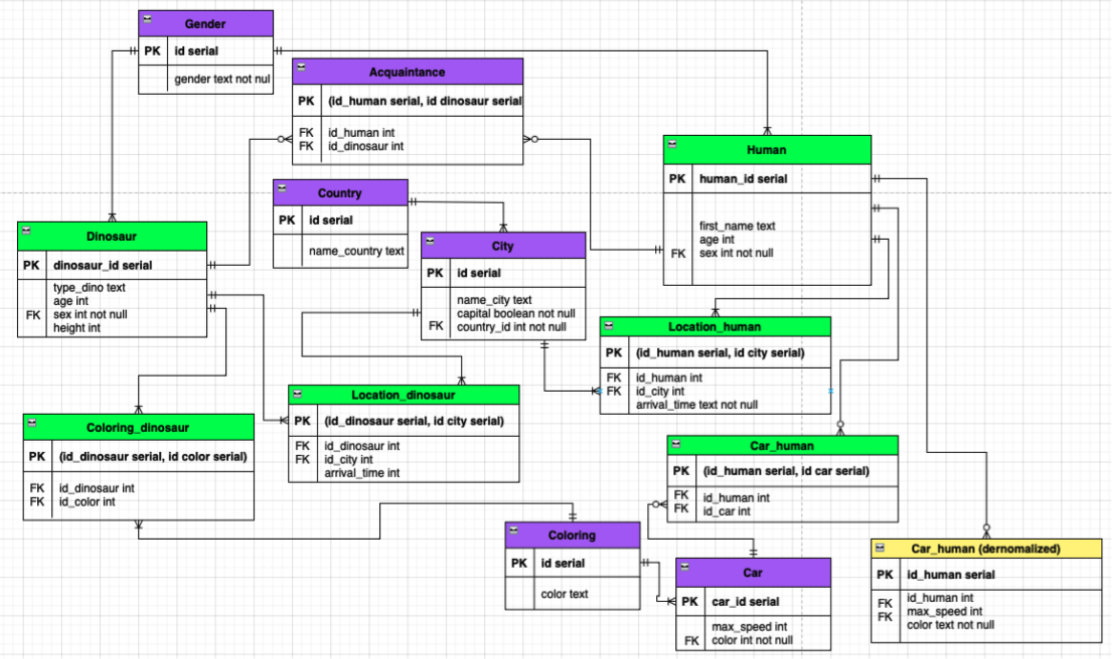
\includegraphics[width=.9\textwidth]{123}